\documentclass[dvisvgm,tikz,border=4pt]{standalone}\usepackage{amsmath,amssymb}
\usetikzlibrary{arrows.meta,decorations.markings,backgrounds,cd,calc}
\colorlet{c1}{blue!70!black}\colorlet{c2}{red!70!black}\colorlet{c3}{green!45!black}
\tikzset{
 ->-/.style={decoration={markings,mark=at position .55 with {\arrow{Stealth[length=2.4mm]}}},postaction={decorate}},
 ->>-/.style={decoration={markings,mark=at position .5 with {\arrow{Stealth[length=2.4mm]}},mark=at position .6 with {\arrow{Stealth[length=2.4mm]}}},postaction={decorate}},
 every picture/.append style={show background rectangle, background rectangle/.style={fill=white}}
}

\begin{document}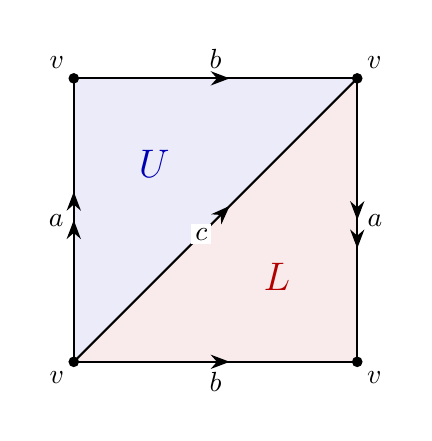
\begin{tikzpicture}[scale=1.2]
\fill[c1!8] (0,0)--(0,3)--(3,3)--cycle; \fill[c2!8] (0,0)--(3,0)--(3,3)--cycle;
\draw[thick,->-] (0,0)--(3,0) node[midway,below]{$b$};
\draw[thick,->-] (0,3)--(3,3) node[midway,above]{$b$};
\draw[thick,->>-] (0,0)--(0,3) node[midway,left]{$a$};
\draw[thick,->>-] (3,3)--(3,0) node[midway,right]{$a$};
\draw[thick,->-] (0,0)--(3,3) node[pos=.45,fill=white,inner sep=1.5pt]{$c$};
\foreach \p in {(0,0),(3,0),(0,3),(3,3)} \fill \p circle(1.6pt);
\node[below left] at (0,0){$v$};\node[below right] at (3,0){$v$};\node[above left] at (0,3){$v$};\node[above right] at (3,3){$v$};
\node[c1,font=\Large] at (0.85,2.1){$U$}; \node[c2,font=\Large] at (2.15,0.9){$L$};
\end{tikzpicture}\end{document}
